
\subsubsection{Zakazivanje isporuka}

\begin{itemize}
	\item Kratak opis:
		\begin{itemize}
			\item Koordinator pravi raspored dostavljačima.
		\end{itemize}
	\item Učesnici:
		\begin{itemize}
		    \item Koordinator
		\end{itemize}
	\item Preduslovi:
		\begin{itemize}
		    \item Postoji bar jedan dostupan dostavljač.
		    \item Sistem je u funkciji.
		\end{itemize}
	\item Postuslovi:
		\begin{itemize}
			\item Svaka narudžbina je dodeljena nekom od dostavljača.
	\end{itemize}
	\item Glavni tok:
		\begin{enumerate}
            \item Koordinator pristupa sistemu i prolazi kroz sve narudžbine koje bi trebalo da se obave sledeće nedelje.
           \item Koordinator svakoj narudžbini dodeljuje dostavljača.
            \item Koordinator dostavljačima preko sistema prosleđuje njegovu listu isporuka za narednu nedelju.
            \item Sistem krajnjem korisniku šalje automatski mejl kojim ga obaveštava da je porudžbina obrađena i podseća  ga u koje vreme mora da bude kod kuće da bi primio porudžbinu.
		\end{enumerate}
   \item Dodatne informacije:
        \begin{itemize}
            \item Lista isporuka se sastoji od identifikacionih brojeva narudžbina i zakazanog vremena dostave za svaku od njih. 
        \end{itemize}
\end{itemize}

\begin{figure}[H]
\begin{center}
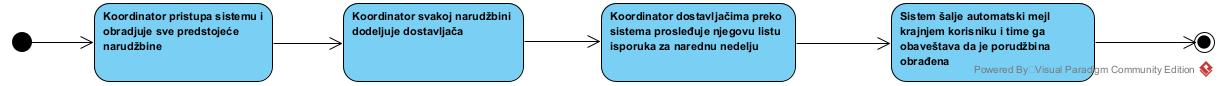
\includegraphics[width=\textwidth]{activity_diagram_scheduling_deliveries.jpg}
\end{center}
    \caption{Dijagram aktivnosti - Zakazivanje isporuka}
\label{fig:Activity_diagram_scheduling_deliveries}
\end{figure}

